\documentclass{article}
\usepackage{fontspec} %Lualatex package
\usepackage{graphicx}

%----------------------------------------------------------------------------------------
% PRINT CODE IN LATEX DOCUMENT
\usepackage{listings}
\lstdefinestyle{fixprintcode}{
    basicstyle=\ttfamily\footnotesize,
    breakatwhitespace=false,
    breaklines=true,
    captionpos=b,
    keepspaces=true,
    numbers=none,
    showspaces=false,
    showstringspaces=false,
    showtabs=false,
    tabsize=2,
    frame=trBL}

    \lstset{style=fixprintcode}

%----------------------------------------------------------------------------------------
% CONFIGURATION OF TIKZ
\usepackage{tikz}
\usetikzlibrary{shapes.geometric, arrows}

% Configuration of Tikz FlowChart
\tikzstyle{startstop} = [rectangle, rounded corners, minimum width=3cm, minimum height=1cm,text centered, draw=black]

\tikzstyle{arrow} = [thick,->,>=stealth]
\tikzstyle{doublearrow} = [densely dotted,<->,>=stealth]
\tikzstyle{dotted} = [loosely dotted,>=stealth]

%----------------------------------------------------------------------------------------
% PREAMBLE OF TABLE AND LIST

\usepackage{tabularx}
\usepackage{booktabs} % Required for better horizontal rules in tables
%\usepackage{multirow}

\usepackage{paralist} %Inline list(inparaenum), always on top of enumitem
\usepackage{longtable} % Enable table cross multiple page
\usepackage{array} %Mostly formatting columns and spacing
\usepackage{enumitem} % Required for list customisation

\setlist{noitemsep} % No spacing between list items
\setlist[itemize]{label=\textbullet, nosep, topsep=0pt, partopsep=0pt, parsep=0pt} % No spacing between itemize

% Remove spacing between itemize env. inside table env.
\makeatletter
% Enumerated columns
\newcolumntype{e}[1]{%
    >{\minipage[t]{\linewidth}\let\\\tabularnewline
      \enumerate
      \addtolength{\rightskip}{0pt plus 50pt}% for raggedright
      \setlength{\itemsep}{-\parsep}}%
    p{#1}%
    <{\@finalstrut\@arstrutbox\endenumerate\endminipage}}

% Itemized columns
\newcolumntype{i}[1]{%
    >{\minipage[t]{\linewidth}\let\\\tabularnewline
      \itemize
      \addtolength{\rightskip}{0pt plus 50pt}% for raggedright
      \setlength{\itemsep}{-\parsep}}%
    p{#1}%
    <{\@finalstrut\@arstrutbox\enditemize\endminipage}}
\makeatother


\begin{document}

\section{Tables and Graphics}
\subsection{FlowChart Sample 1}
This environment should uncomment package of TiKz and also configuration of TiKz flowchart in .cls file.
\begin{lstlisting}[language=TeX, caption=Flowchart sample 1]
\begin{figure}[hp]
\centering
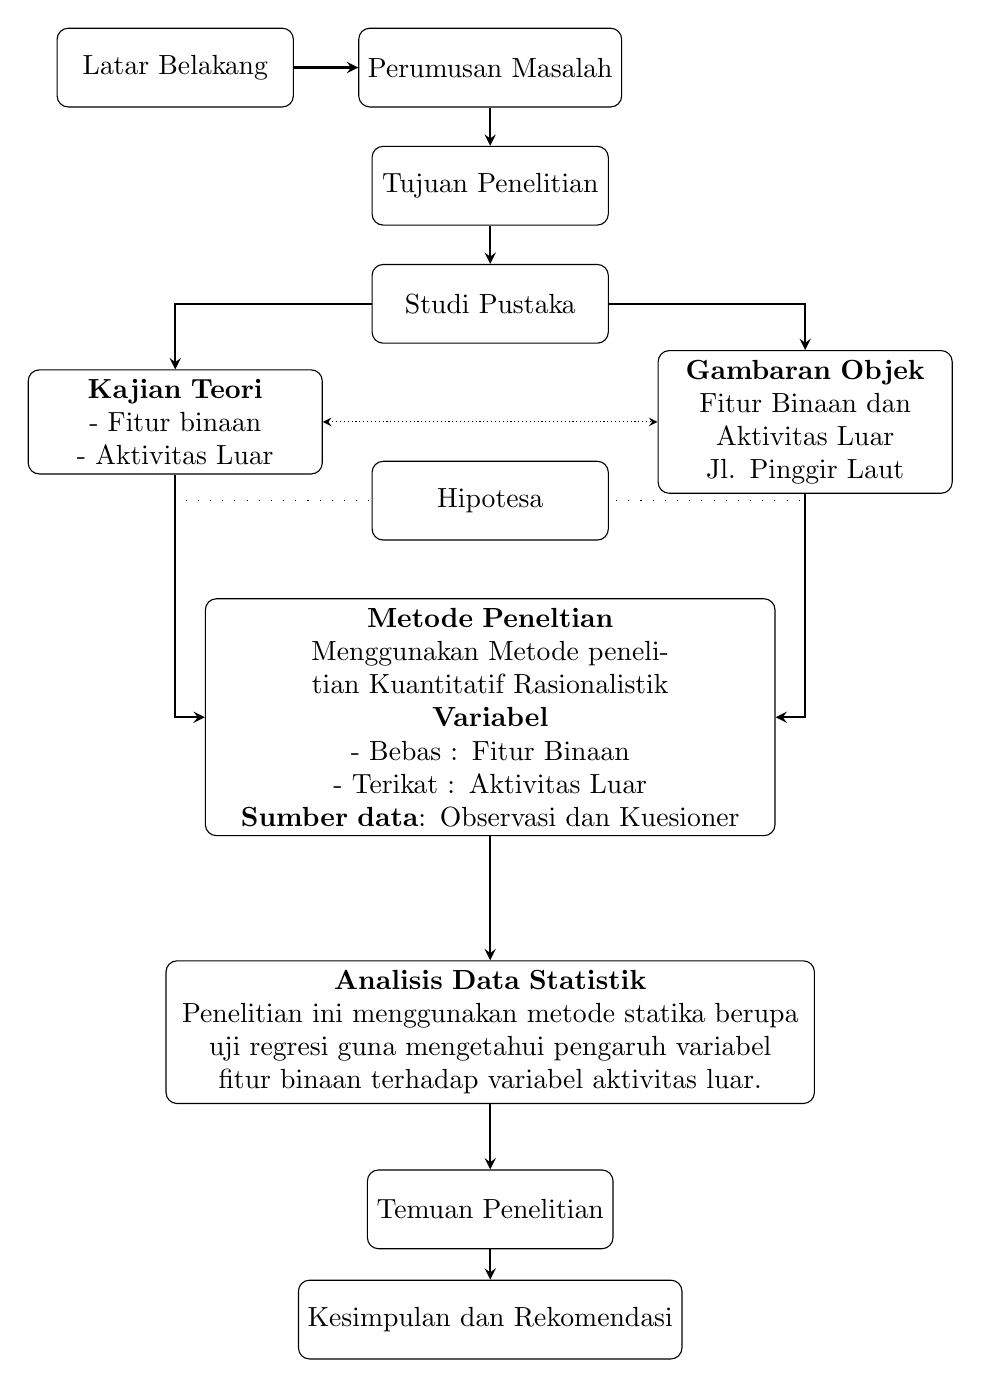
\begin{tikzpicture}[node distance=2cm]

\node (ltr) [startstop] {Latar Belakang};
\node (rum) [startstop, right of=ltr, xshift=2cm] {Perumusan Masalah};
\node (tuj) [startstop, below of=rum, yshift=0.5cm] {Tujuan Penelitian};
\node (pus) [startstop, below of=tuj, yshift=0.5cm] {Studi Pustaka};
\node (kaj) [startstop, below of=pus, text width=3.5cm, xshift= -4cm, yshift=.5cm] {
	\textbf{Kajian Teori}\\ - Fitur binaan\\ - Aktivitas Luar
};
\node (kaj2) [startstop, below of=pus, text width=3.5cm, xshift= 4cm, yshift=.5cm] {
	\textbf{Gambaran Objek}\\ Fitur Binaan dan Aktivitas Luar Jl. Pinggir Laut
};
\node (hip) [startstop, below of=pus, yshift=-.5cm] {Hipotesa};
\node (met) [startstop, below of=hip, yshift=-.75cm, text width=7cm] {
	\textbf{Metode Peneltian}\\ Menggunakan Metode penelitian Kuantitatif Rasionalistik

	\textbf{Variabel}\\
	- Bebas : Fitur Binaan\\
	- Terikat : Aktivitas Luar\\

	\textbf{Sumber data}: Observasi dan Kuesioner
};
\node (ana) [startstop, below of=met, text width=8cm, yshift=-2cm] {
		\textbf{Analisis Data Statistik}\\ Penelitian ini menggunakan metode statika berupa uji regresi guna mengetahui pengaruh variabel fitur binaan terhadap variabel aktivitas luar.
};
\node (tem) [startstop, below of=ana, yshift=-.25cm] {Temuan Penelitian};
\node (kes) [startstop, below of=tem, yshift=.6cm] {Kesimpulan dan Rekomendasi};

\draw [arrow] (ltr) -- (rum);
\draw [arrow] (rum) -- (tuj);
\draw [arrow] (tuj) -- (pus);
\draw [arrow] (pus) -| (kaj);
\draw [arrow] (pus) -| (kaj2);
\draw [doublearrow] (kaj) -- (kaj2);
\draw [arrow] (kaj) |- (met);
\draw [dotted] (kaj) |- (hip);
\draw [arrow] (kaj2) |- (met);
\draw [dotted] (kaj2) |- (hip);
\draw [arrow] (met) -- (ana);
\draw [arrow] (ana) -- (tem);
\draw [arrow] (tem) -- (kes);

\end{tikzpicture}
\caption{Alur Pikir}
\end{figure}
\end{lstlisting}

%-----------------------------------------------------------------------------------
% 	[[REAL CODE]]
%----------------------------------------------------------------------------------
\begin{figure}[hp]
\centering
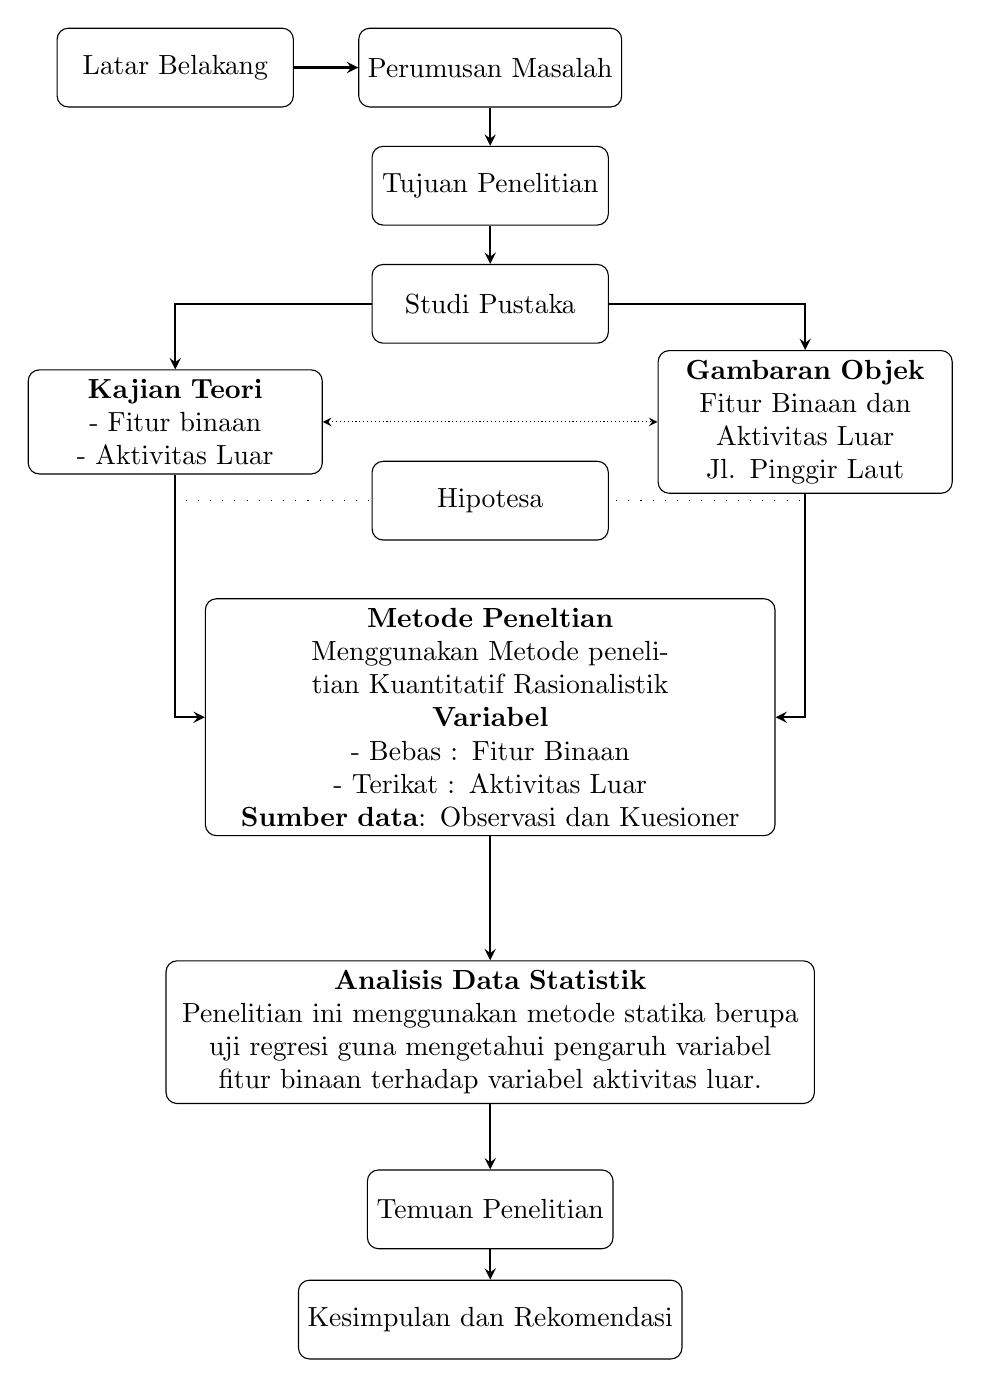
\begin{tikzpicture}[node distance=2cm]

\node (ltr) [startstop] {Latar Belakang};
\node (rum) [startstop, right of=ltr, xshift=2cm] {Perumusan Masalah};
\node (tuj) [startstop, below of=rum, yshift=0.5cm] {Tujuan Penelitian};
\node (pus) [startstop, below of=tuj, yshift=0.5cm] {Studi Pustaka};
\node (kaj) [startstop, below of=pus, text width=3.5cm, xshift= -4cm, yshift=.5cm] {
	\textbf{Kajian Teori}\\ - Fitur binaan\\ - Aktivitas Luar
};
\node (kaj2) [startstop, below of=pus, text width=3.5cm, xshift= 4cm, yshift=.5cm] {
	\textbf{Gambaran Objek}\\ Fitur Binaan dan Aktivitas Luar Jl. Pinggir Laut
};
\node (hip) [startstop, below of=pus, yshift=-.5cm] {Hipotesa};
\node (met) [startstop, below of=hip, yshift=-.75cm, text width=7cm] {
	\textbf{Metode Peneltian}\\ Menggunakan Metode penelitian Kuantitatif Rasionalistik

	\textbf{Variabel}\\
	- Bebas : Fitur Binaan\\
	- Terikat : Aktivitas Luar\\

	\textbf{Sumber data}: Observasi dan Kuesioner
};
\node (ana) [startstop, below of=met, text width=8cm, yshift=-2cm] {
		\textbf{Analisis Data Statistik}\\ Penelitian ini menggunakan metode statika berupa uji regresi guna mengetahui pengaruh variabel fitur binaan terhadap variabel aktivitas luar.
};
\node (tem) [startstop, below of=ana, yshift=-.25cm] {Temuan Penelitian};
\node (kes) [startstop, below of=tem, yshift=.6cm] {Kesimpulan dan Rekomendasi};

\draw [arrow] (ltr) -- (rum);
\draw [arrow] (rum) -- (tuj);
\draw [arrow] (tuj) -- (pus);
\draw [arrow] (pus) -| (kaj);
\draw [arrow] (pus) -| (kaj2);
\draw [doublearrow] (kaj) -- (kaj2);
\draw [arrow] (kaj) |- (met);
\draw [dotted] (kaj) |- (hip);
\draw [arrow] (kaj2) |- (met);
\draw [dotted] (kaj2) |- (hip);
\draw [arrow] (met) -- (ana);
\draw [arrow] (ana) -- (tem);
\draw [arrow] (tem) -- (kes);

\end{tikzpicture}
\caption{Flowchart sample 1}
\end{figure}


\subsection{Flowchart Sample 2 }

\begin{lstlisting}[language=TeX, caption=Flowchart sample 2]
\begin{figure}[htbp]
\centering
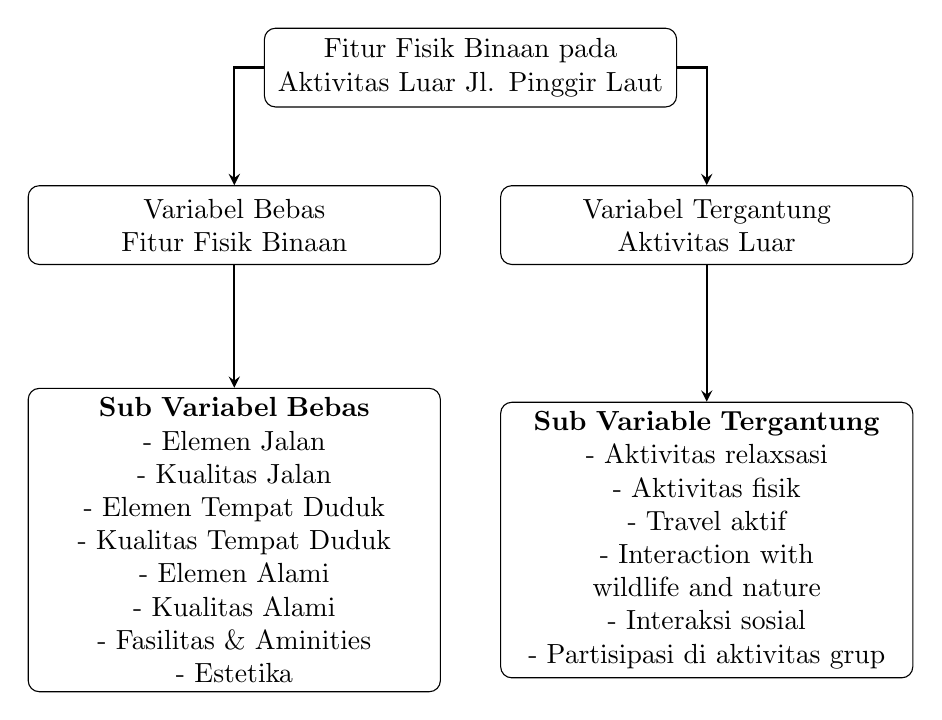
\begin{tikzpicture}[node distance=2cm]

	\node (tit) [startstop, text width= 5cm] {Fitur Fisik Binaan pada Aktivitas Luar Jl. Pinggir Laut};
	\node (va1) [startstop, below of=tit, text width=5cm, xshift=-3cm] {Variabel Bebas\\ Fitur Fisik Binaan};
	\node (va2) [startstop, below of=tit, text width=5cm, xshift=3cm] {Variabel Tergantung\\ Aktivitas Luar};
	\node (de1) [startstop, below of=va1, text width=5cm, yshift=-2cm] {
		\textbf{Sub Variabel Bebas}\\
		- Elemen Jalan \\
		- Kualitas Jalan \\
		- Elemen Tempat Duduk \\
		- Kualitas Tempat Duduk \\
		- Elemen Alami \\
		- Kualitas Alami \\
		- Fasilitas \& Aminities \\
		- Estetika \\
	};
	\node (de2) [startstop, below of=va2, text width=5cm, yshift=-2cm] {
			\textbf{Sub Variable Tergantung}\\
		- Aktivitas relaxsasi\\
		- Aktivitas fisik\\
		- Travel aktif\\
		- Interaction with wildlife and nature\\
		- Interaksi sosial\\
		- Partisipasi di aktivitas grup\\
		};

\draw [arrow] (tit) -| (va1);
\draw [arrow] (va1) -- (de1);
\draw [arrow] (tit) -| (va2);
\draw [arrow] (va2) -- (de2);

\end{tikzpicture}
\caption{Alur Pikir}
\end{figure}
\end{lstlisting}
%-----------------------------------------------------------------------------------
% 	[[REAL CODE]]
%----------------------------------------------------------------------------------
\begin{figure}[htbp]
\centering
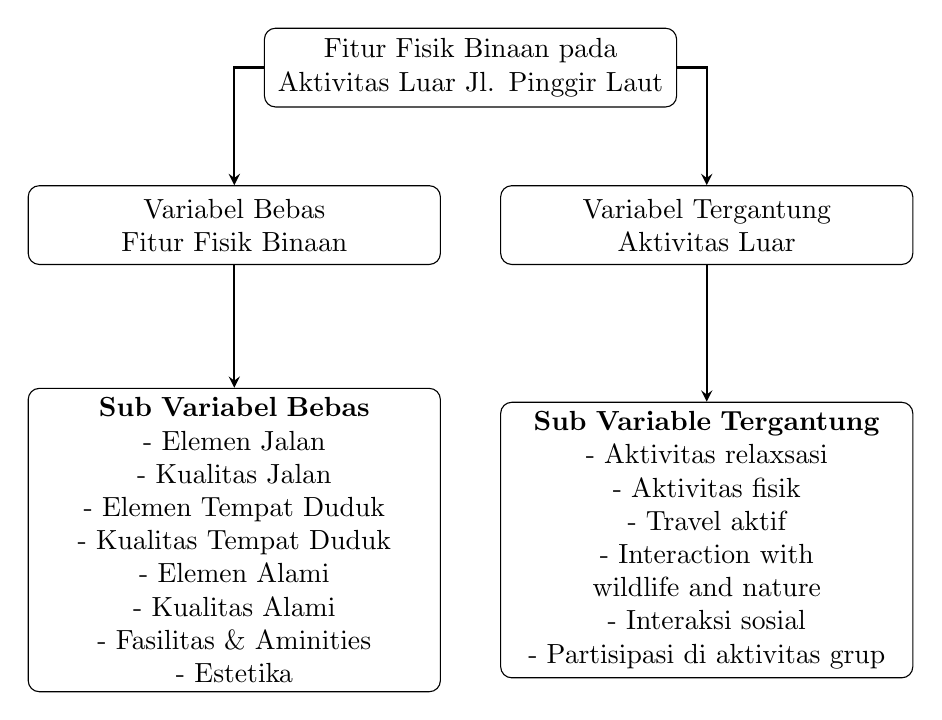
\begin{tikzpicture}[node distance=2cm]

	\node (tit) [startstop, text width= 5cm] {Fitur Fisik Binaan pada Aktivitas Luar Jl. Pinggir Laut};
	\node (va1) [startstop, below of=tit, text width=5cm, xshift=-3cm] {Variabel Bebas\\ Fitur Fisik Binaan};
	\node (va2) [startstop, below of=tit, text width=5cm, xshift=3cm] {Variabel Tergantung\\ Aktivitas Luar};
	\node (de1) [startstop, below of=va1, text width=5cm, yshift=-2cm] {
		\textbf{Sub Variabel Bebas}\\
		- Elemen Jalan \\
		- Kualitas Jalan \\
		- Elemen Tempat Duduk \\
		- Kualitas Tempat Duduk \\
		- Elemen Alami \\
		- Kualitas Alami \\
		- Fasilitas \& Aminities \\
		- Estetika \\
	};
	\node (de2) [startstop, below of=va2, text width=5cm, yshift=-2cm] {
			\textbf{Sub Variable Tergantung}\\
		- Aktivitas relaxsasi\\
		- Aktivitas fisik\\
		- Travel aktif\\
		- Interaction with wildlife and nature\\
		- Interaksi sosial\\
		- Partisipasi di aktivitas grup\\
		};

\draw [arrow] (tit) -| (va1);
\draw [arrow] (va1) -- (de1);
\draw [arrow] (tit) -| (va2);
\draw [arrow] (va2) -- (de2);

\end{tikzpicture}
\caption{Flowchart sample 2}
\end{figure}



\subsection{Longtable Sample}
This is a sample of longtable with itemize environment. Spacing between environment of itemize being reduced. This environment required longtable,array and enumitem packages. Minipage configuration with command multicolumn has no effect from set spacing in itemize.

\begin{lstlisting}[language=TeX, caption=Table sample 1]
\begin{longtable}{p{.5\textwidth} p{.5\textwidth}}
	\caption{Caption} \\
	\label{tab:label} \\
	text & \multicolumn{1}{i{.4\textwidth}}{\item text \item text}\\

\end{longtable}
\end{lstlisting}

%-----------------------------------------------------------------------------------
% 	[[REAL CODE]]
%----------------------------------------------------------------------------------
\begin{longtable}{p{.5\textwidth} p{.5\textwidth}}
	\caption{Longtable sample 1} \\
	\label{tab:label} \\
	text & \multicolumn{1}{i{.4\textwidth}}{\item text \item text}\\

\end{longtable}

%\section{readme}
%\lipsum[11-12]
% Comment tikz flowchart with command :x,xxs/^/%
% Uncomment tikz flowchart with command :x,xxs/^%/
% xx = linenumbers


\end{document}

